\documentclass[10pt,fleqn]{article} % Default font size and left-justified equations
\usepackage[%
    pdftitle={Equilibrage des solides en rotation},
    pdfauthor={Xavier Pessoles}]{hyperref}

\input{style/new_style}
\input{style/macros_SII}
\usepackage{bm}
\fichetrue
\fichefalse

\proftrue
%\proffalse

%\tdtrue
\tdfalse

\courstrue
%\coursfalse



% -------------------------------------
% Déclaration des titres
% -------------------------------------

\def\discipline{Sciences \\Industrielles de \\ l'Ingénieur}
\def\xxtete{Sciences Industrielles de l'Ingénieur}

\def\classe{\textsf{PSI$\star$ -- MP}}
\def\xxnumpartie{Cycle 06}
\def\xxpartie{Équilibrage des solides en rotation}

\def\xxnumchapitre{Chapitre 1 \vspace{.2cm}}
\def\xxchapitre{\hspace{.12cm} Équilibrage des solides en rotation}

\def\xxposongletx{2}
\def\xxposonglettext{1.45}
\def\xxposonglety{19}%16

\def\xxonglet{\textsf{Cycle 06}}

\def\xxactivite{Cours}
\def\xxauteur{\textsl{Emilien Durif}}

\def\xxcompetences{%
\textsl{%
\textbf{Savoirs et compétences :}\\
\begin{itemize}[label=\ding{112},font=\color{ocre}] 
\item \textit{Mod2.C16} : torseur cinétique
\item \textit{Mod2.C17} : torseur dynamique
\item \textit{Mod2.C17.SF1} : déterminer le torseur dynamique d’un solide, ou d’un ensemble de solides, par rapport à un autre solide
\item \textit{Mod2.C15} : matrice d'inertie
\item \textit{Res1.C2} : principe fondamental de la dynamique
\item \textit{Res1.C1.SF1} : proposer une démarche permettant la détermination de la loi de mouvement
\item \textit{Res1.C2.SF1} : proposer une méthode permettant la détermination d’une inconnue de liaison
\end{itemize}
}}
		



\def\xxfigures{
\includegraphics[width=0.4\textwidth]{images/turbine_alstom.jpeg}\\
\textit{Turbine à gaz Alstom}

\includegraphics[width=0.5\textwidth]{images/turboreacteur.jpeg}\\
\textit{Turborécateur Snecma}

}%figues de la page de garde

\def\xxpied{%
Cycle 06 -- Équilibrage des solides en rotation\\% afin de valider leurs performances.\\
Chapitre 1 -- \xxactivite%
}

\setcounter{secnumdepth}{5}
%---------------------------------------------------------------------------


\begin{document}
\chapterimage{png/Fond_CIN}
\input{style/new_pagegarde}
\setlength{\columnseprule}{.1pt}

\vspace{2cm}
\pagestyle{fancy}
\thispagestyle{plain}
%%%%%%%%%%%%%%%%%%%%%%%%%%%%%%%%%%%ù




\section{Introduction}
\subsection{Problématique industrielle}

Le mise en rotation de rotor à haute vitesse (à partir de quelques centaines de tours par minute) est une configuration classique rencontrée dans l'industrie. Si un défaut géométrique existe, cela induit une dissymétrie de la répartition de masse qui provoque des effets vibratoires pouvant aller jusqu'à la rupture des éléments de guidage (paliers, roulements à billes).

Afin d'éviter ces problèmes il convient d'équilibrer dynamiquement ces rotors ce qui implique de rendre les actions mécaniques au niveau des guidages en rotation constantes au cours du temps.
%
%%\begin{figure}[!htbf]
%\begin{center}
%\begin{tabular}{cc}
%\includegraphics[width=0.4\textwidth]{images/turbine_alstom.jpeg}
%&
%\includegraphics[width=0.5\textwidth]{images/turboreacteur.jpeg}\\
%Turbine à gaz Alstom & Turborécateur Snecma
%\end{tabular}
%%\caption{Exemple de systèmes présentant des structures tournantes à haute vitesse \label{exemple_rotor}}
%\textit{Exemple de systèmes présentant des structures tournantes à haute vitesse \label{exemple_rotor}}
%\end{center}
%%\end{figure}

\subsection{Présentation du support de cours}

\begin{exemple}[Étude d'une pompe turbo-moléculaire]
On s'intéresse ici à l'étude d'une pompe à vide destinée à la fabrication de composants électroniques capable d'évacuer des gaz en créant un vide de l'ordre $10^{-9}\,\text{mbar}$ dans une chambre blanche. Les conditions du cahier des charges sont très exigeantes et résumées dans le diagramme des exigences partiel suivant : 

\begin{center}
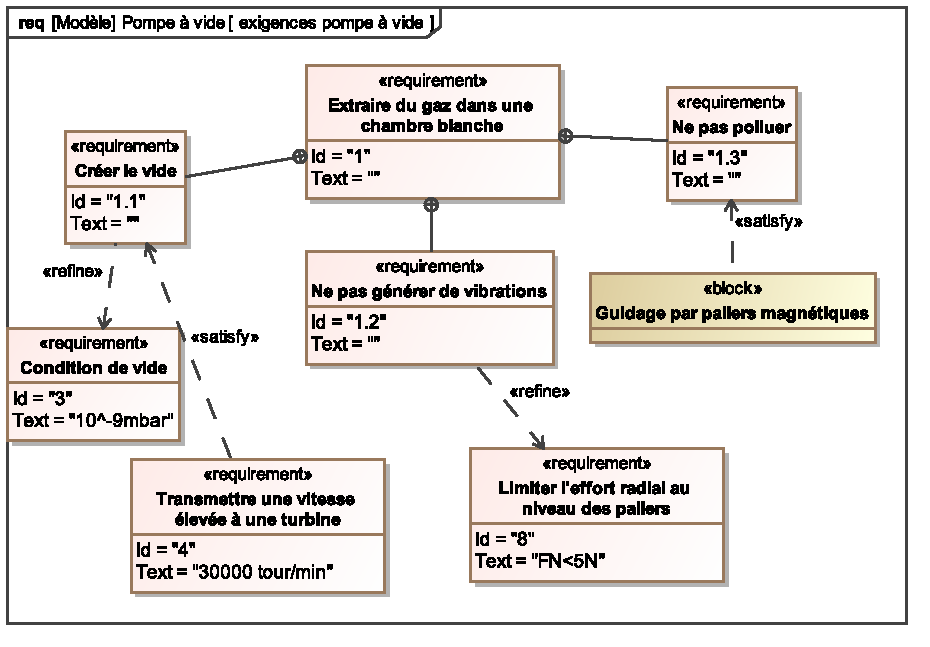
\includegraphics[width=0.9\textwidth]{images/req_pompe.pdf}\\
\textbf{Diagramme des exigences partiel de la pompe à vide}
\end{center}
\end{exemple}

%\begin{figure}[!htbf]
\begin{center}
\begin{tabular}{cc}
\includegraphics[width=0.3\textwidth]{images/rotor_pompe.jpg}
&
\includegraphics[width=0.5\textwidth]{images/guidage_pompe.jpg}
\\
Rotor de la pompe
&
Vue en coupe du guidage par paliers magnétiques de la pompe
\end{tabular}
\end{center}
%\end{figure}





\section{Modélisation du problème}
\subsection{Paramétrage du problème}

\begin{multicols}{2}
La figure ci-dessous représente le paramétrage d'un rotor $S_3$ en mouvement par rapport à $S_0$.

%\begin{figure}[htbf!]
\begin{center}
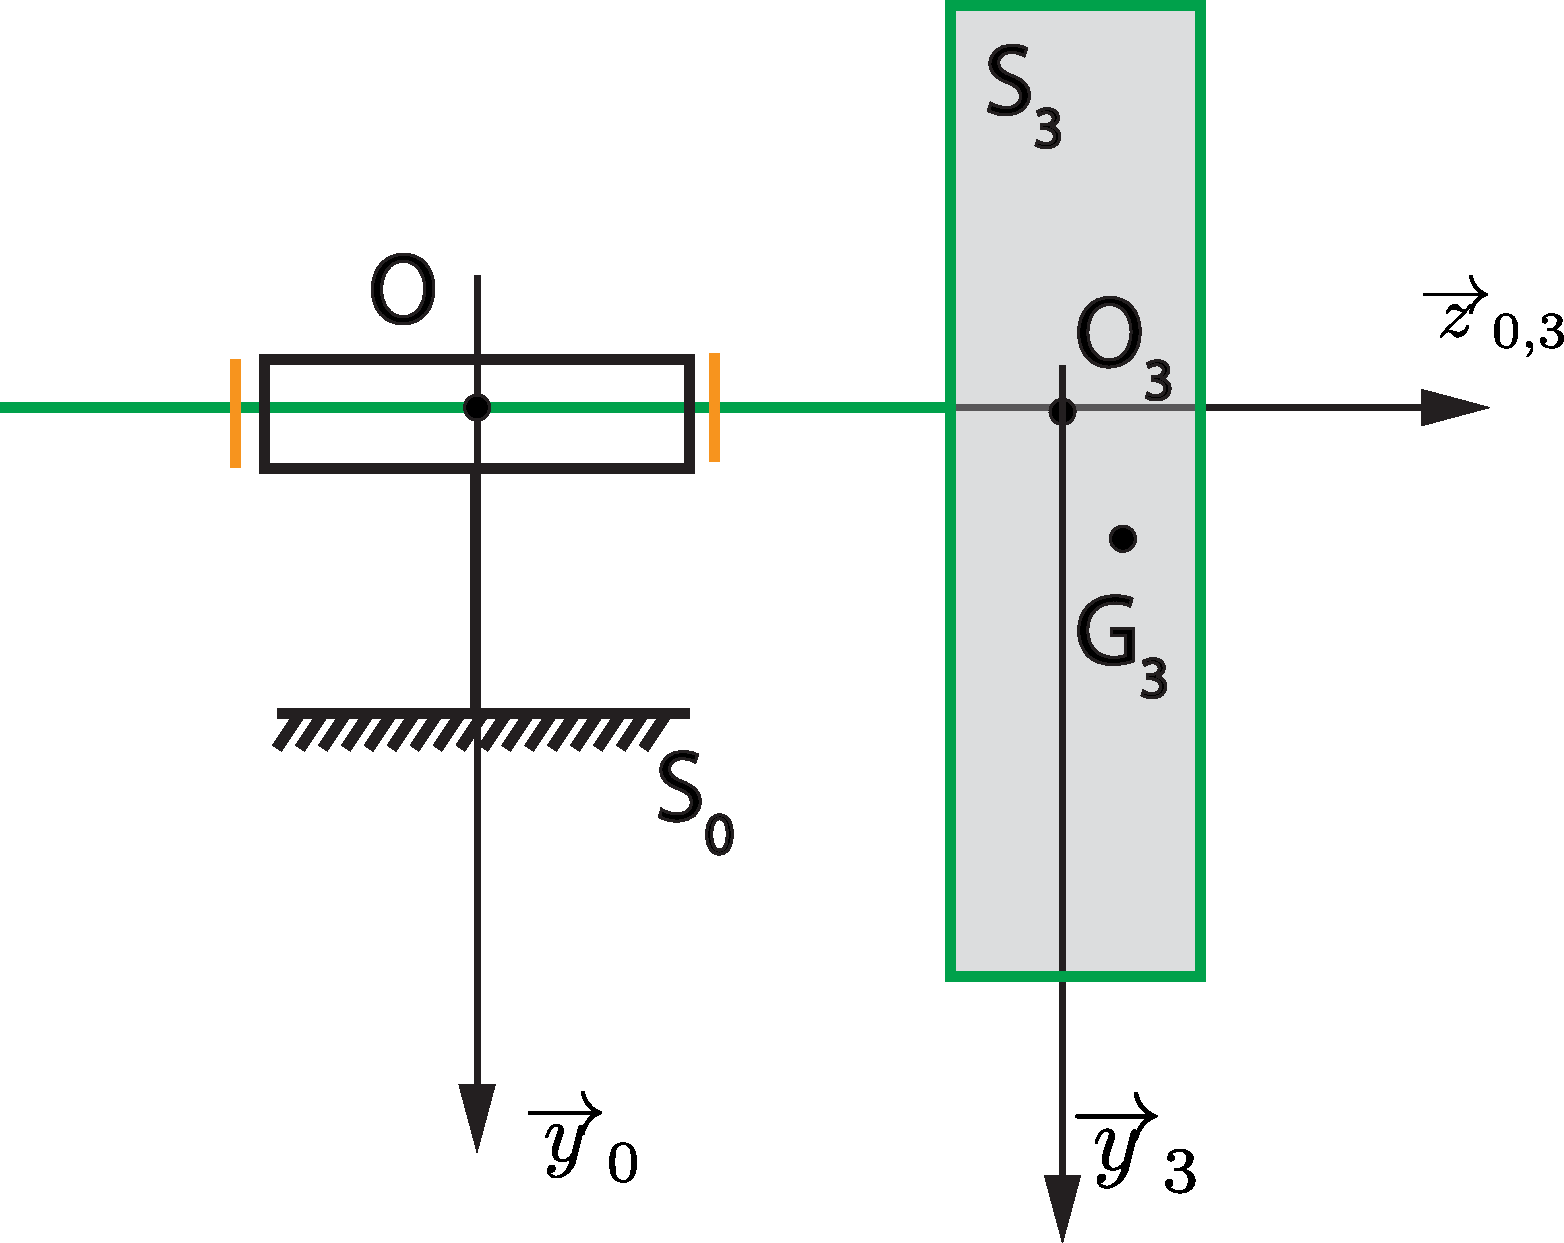
\includegraphics[width=.8\linewidth]{images/figure_presentation.pdf}
%%%\scFigCalc[z_{0,3}]{x_0}{y_0}{x_3}{y_3}{\theta}
\includegraphics[width=.4\linewidth]{images/sc}
\end{center}
%\caption{Paramétrage du problème}
\textit{Paramétrage du problème}
%\end{figure}



\begin{itemize}
\item Le référentiel $R_0$ associé à $S_0$ est supposé comme étant galiléen.
\item Le guidage par paliers magnétiques entre le rotor $S_3$ et le bâti $S_0$ est modélisé par une liaison pivot d'axe ($O_3$,$\vect{z}_{0,3}$) avec bâti $S_0$.
\item Le paramètre du mouvement de $S_3/S_0$ est défini par $\theta=(\vect{x_0},\vect{x_3})$.
\item Le rotor $S_3$ est de masse $m_3$, de centre de masse $G_3$ tel que $\vect{O_3G_3}=b \vect{y_3}+c\vect{z_3}$.
\item Le rotor $S_3$, bien qu'ayant une symétrie théorique de révolution est en réalité imparfait. Sa matrice d'inertie en $O_3$ est donnée par :
$$
\overline{\overline{I}}_{O_3}(S_3)=\left(\begin{array}{ccc}
A_3 & -F_3 & -E_3 \\ 
-F_3 & B_3 & -D_3 \\ 
-E_3 & -D_3 & C_3
\end{array} \right)_{R_3}
$$
\item Un moteur, non représenté, entraîne $S_3$ avec un couple $C_m \vect{z_{0,3}}$ à vitesse constante ($\omega=\dot{\theta}$).
\item L'accélération de la pesanteur est dirigée selon $+\vect{y_0}$ et vaut $g=\SI{9,81}{m.s^{-2}}$.
\end{itemize}
\end{multicols}

\subsection{Analyse préliminaire}
%\begin{exemple}[Analyse préliminaire]
%\subparagraph{}
\textit{Faire le bilan des actions mécaniques extérieures pour $\left\{S_3\right\}$.}
%\begin{texteCache}
\begin{itemize}
\item \textbf{Action du bâti (liaison pivot)} :
$
\torseurstat{T}{S_0}{S_3}
=\torseurl{X_{03} \vect{x_{0}}+ Y_{03} \vect{y_{0}}+Z_{03} \vect{z_{0}}}{L_{03} \vect{x_{0}}+M_{03} \vect{y_{0}}}{\forall P\in \couple{O_3}{z_{0,3}}}
$
\item \textbf{Action du moteur : }
$
\torseurstat{T}{\text{moteur}}{S_3}
=\torseurl{\vect{0}}{C_{m} \vect{z_0}}{\forall P}
$.
\item \textbf{Action de la pesanteur : }
$
\torseurstat{T}{\text{pesanteur}}{S_3}
=\torseurl{m_3 g \vect{y_0}}{\vect{0}}{G_3}\\
=\torseurl{m_3 g \vect{y_0}}{\vect{O_3G_3}\wedge \left(m_3 g \vect{y_0}\right)=\left(b \vect{y_3}+c\vect{z_3}\right)\wedge\left(m_3 g \vect{y_0}\right)}{O_3}
=\torseurl{m_3 g \vect{y_0}}{m_3 g\left(-b\sin\theta \vect{z_{0,3}} -c\vect{x_0}\right)}{O_3}\\
$
\end{itemize}

%\end{texteCache}

%\subparagraph{}
\textit{Déterminer le torseur dynamique $\torseurdyn{S_3}{R_0}$ en $O_3$.}

\begin{itemize}
\item Le solide $S_3$ est en mouvement de rotation autour de l'axe $\couple{O_3}{z_{0,3}}$ fixe par rapport à $R_0$.

%\begin{texteCache}
\begin{align*}
\torseurdyn{S_3}{R_0}=
\torseurl{
\vect{R_d}(S_3/R_0)=m_3 \vect{a}(G_3\in S_3/R_0)}{
\vectmd{O_3}{S_3}{R_0}=\left[\frac{\dd \vectmc{O_3}{S_3}{R_0}}{\dd t}\right]_{R_0}}{O_3}
\end{align*}
%\end{texteCache}

\item On calcule $\vect{R_d}(S_3/R_0)$ : 
%\begin{texteCache}
$
\vect{R_d}(S_3/R_0)=m_3 \vect{a}(G_3\in S_3/R_0)
=m_3 \left[\frac{\dd \vect{V}(G_3\in S_3/R_0)}{\dd t}\right]_{R_0}
$.

Or, 
$
\vect{V}(G_3\in S_3/R_0)=\vect{G_3O_3}\wedge \vect{\Omega}(S_3/R_0)=
(-b \vect{y}_3-c \vect{z_3})\wedge \dot{\theta} \vect{z_{0,3}}
=-b \dot{\theta} \vect{x_3}.
$

Donc,

\begin{align*}
\vect{R_d}(S_3/R_0)=-b m_3 \left(\ddot{\theta} \vect{x_3}+\dot{\theta} \left[\frac{\dd  \vect{x_3}}{\dd t}\right]_{R_0}\right)
=-b m_3 \left(\ddot{\theta} \vect{x_3}+\dot{\theta}^2 \vect{y_3}\right)\\
=-b m_3 \omega^2 \vect{y_3}=-b m_3 \omega^2\left(-\sin\theta \vect{x_0}+\cos\theta \vect{y_0}\right)
\end{align*}

%\end{texteCache}

\item On calcule $\vectmc{O_3}{S_3}{R_0}$.
%\begin{texteCache}
$O_3$ est fixe par rapport à $R_0$ : 
$
\vectmc{O_3}{S_3}{R_0}=\overline{\overline{I}}_{O_3}(S_3) \vect{\Omega}(S_3/R_0)
=\left(\begin{array}{ccc}
A_3 & -F_3 & -E_3 \\ 
-F_3 & B_3 & -D_3 \\ 
-E_3 & -D_3 & C_3
\end{array} \right)_{R_3}\cdot
\left(\begin{array}{c}
0 \\ 
0 \\ 
\dot{\theta}
\end{array} \right)_{R_3}
=\dot{\theta}\left(-E_3 \vect{x_3}-D_3 \vect{y_3}+C_3 \vect{z_3}\right)
$
%\end{texteCache}
\end{itemize}
%\end{exemple}

%\setcounter{cptExemple}{\thecptExemple-1}
%\begin{exemple}[Analyse préliminaire]
\begin{itemize}
\item On calcule $\vectmd{O_3}{_3}{R_0}$ : 
%\begin{texteCache}
$O_3$ est fixe par rapport à $R_0$ : 
\begin{align*}
\vectmd{O_3}{_3}{R_0}=\left[\frac{\dd \vectmc{O_3}{S_3}{R_0}}{\dd t}\right]_{R_0}
=
\left(-E_3\cdot\ddot{\theta}+D_3 \dot{\theta}^2\right) \vect{x_3}+\left(-D_3\cdot\ddot{\theta}-E_3 \dot{\theta}^2\right) \vect{y_3}+C_3\cdot\ddot{\theta} \vect{z_{0,3}}\\
=D_3 \omega^2 \vect{x}_3-E_3 \omega^2 \vect{y_3}\\
=\omega^2 \left[\left(D_3\cdot\cos\theta+E_3\cdot\sin\theta\right) \vect{x_0}+\left(D_3\cdot\sin\theta-E_3\cdot\cos\theta\right) \vect{y_0}\right]
\end{align*}
%\end{texteCache}

\item On en déduit $\torseurdyn{S_3}{R_0}$ exprimé dans la base $b_0=\base{{x}_0}{{y}_0}{{z}_0}$ : 
%\begin{texteCache}
\begin{align*}
\torseurdyn{S_3}{R_0}
=\torseurl{-b m_3 \omega^2\left(-\sin\theta \vect{x_0}+\cos\theta \vect{y_0}\right)}{\omega^2 \left[\left(D_3\cdot\cos\theta+E_3\cdot\sin\theta\right) \vect{x_0}+\left(D_3\cdot\sin\theta-E_3\cdot\cos\theta\right) \vect{y_0}\right]}{O_3}
\end{align*}
%\end{texteCache}
\end{itemize}

%\subparagraph{}
\textit{Déduire du Principe Fondamental de la Dynamique, les équations de mouvement.}

%\begin{texteCache}
Le Principe Fondamental de la dynamique appliqué à $S_3$ par rapport au référentiel $R_0$ donne :

\begin{multicols}{2}
Théorème de la résultante dynamique : 

$$
\begin{array}{cc}
\begin{array}{c}
\vect{x_0}\\
\vect{y_0}\\
\vect{z_0}
\end{array}
&
\left\{
\begin{array}{c}
X_{03}=b m_3 \omega^2\sin\theta\\
Y_{03}+m_3 g=-b m_3 \omega^2\cos\theta\\
Z_{03}=0
\end{array}
\right.
\end{array}
$$

Théorème du moment dynamique en $O_0$: 
$$
\begin{array}{cc}
\begin{array}{c}
\vect{x_0}\\
\vect{y_0}\\
\vect{z_0}
\end{array}
&
\left\{
\begin{array}{c}
L_{03}=\omega^2 \left(D_3\cdot\cos\theta+E_3\cdot\sin\theta\right)+c m_3 g\\
M_{03}=\omega^2\cdot\left(D_3\cdot\sin\theta-E_3\cdot\cos\theta\right)\\
C_m-m_3 g b\sin\theta=0
\end{array}
\right.
\end{array}
$$
\end{multicols}
%\end{texteCache}

%\end{exemple}


\begin{prop}[Évolution des efforts au niveau des paliers au cours du temps]
Lorsque le rotor n'est pas équilibré dynamiquement (comme dans l'exemple précédent), les actions extérieurs dans la liaison pivot dépendant de la position angulaire et fluctuent cycliquement.

On donne ci-dessous les évolutions des composantes de l'action mécanique dans la liaison pivot pour une rotation du rotor 3:
\begin{itemize}
\item opérateur d'inertie : $E_3=0$ et $D_3=10^{-4}\;\text{kg m}^2$ ; 
\item masse et centre de masse : $m_3=\SI{10}{kg}$, $c=\SI{0}{mm}$ et $b=\SI{0,05}{mm}$ ; 
\item rotation de $3/0$ : $\omega=\SI{30000}{tour/min}$.
\end{itemize}

\begin{center}

\begin{minipage}{0.45\textwidth}
\begin{center}
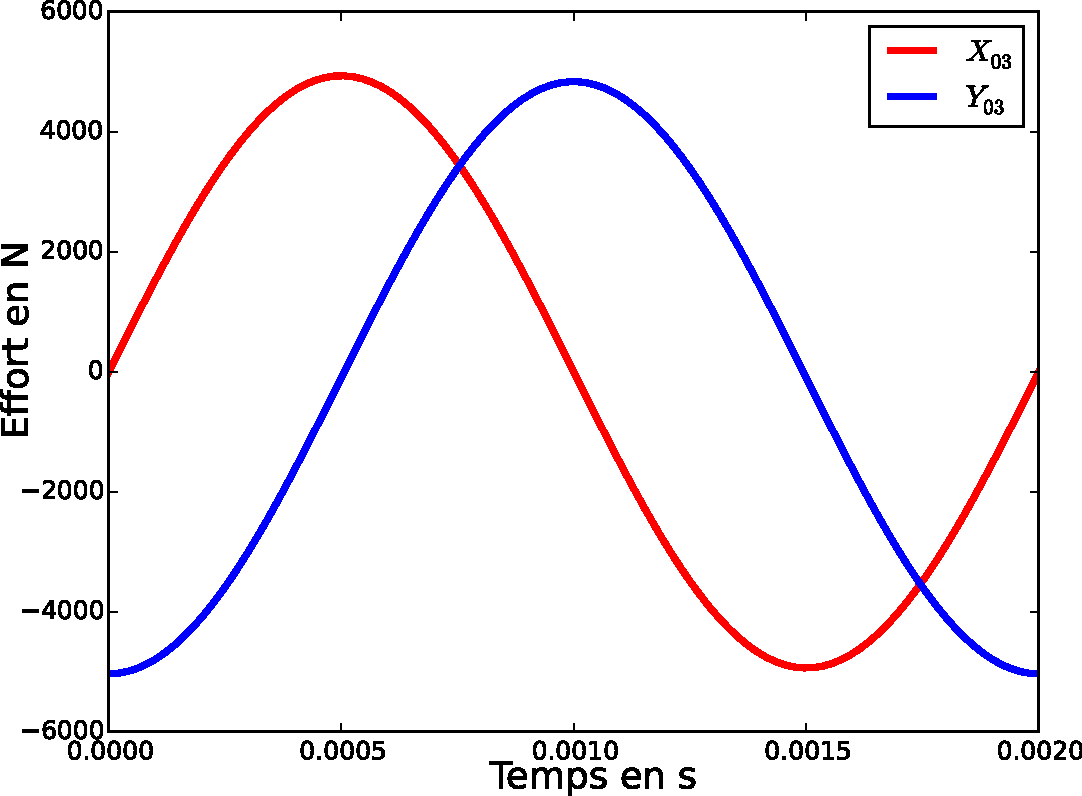
\includegraphics[width=1.0\textwidth]{images/effort.pdf}
\end{center}
\end{minipage}
\begin{minipage}{0.45\textwidth}
\begin{center}
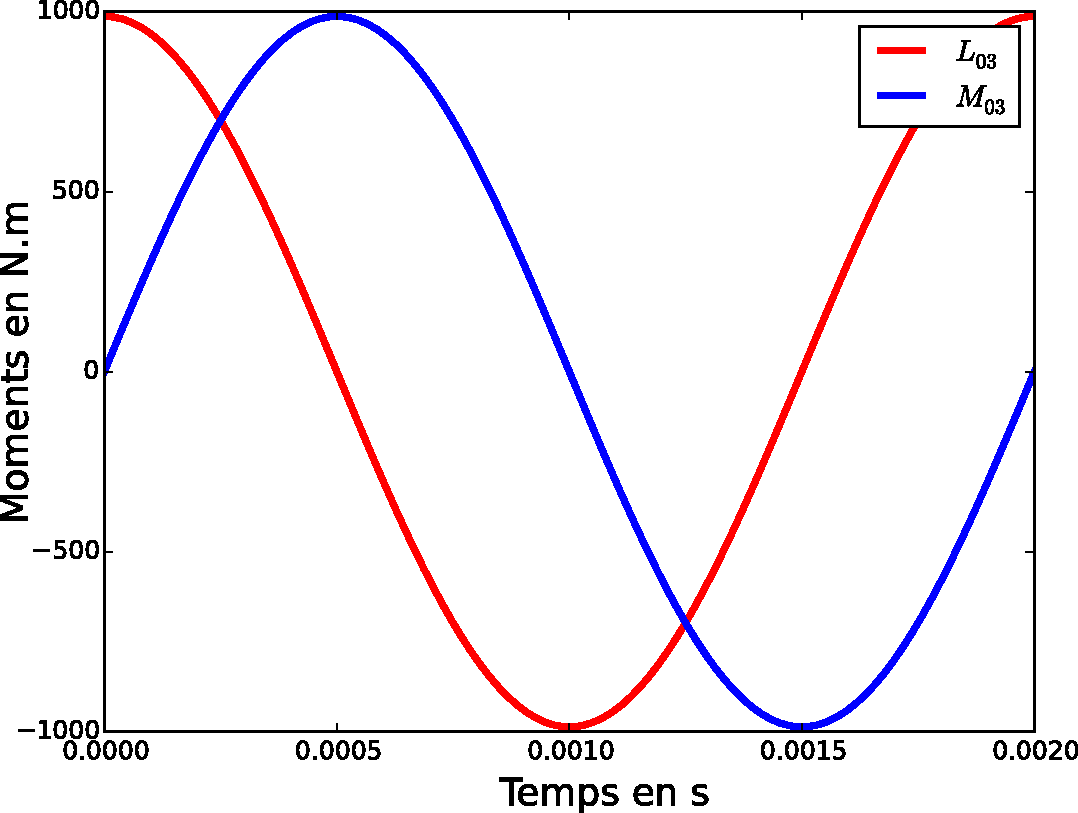
\includegraphics[width=1.0\textwidth]{images/moment.pdf}
\end{center}
\end{minipage}
\end{center}

Il apparaît des variations d'efforts de l'ordre de $\SI{10}{kN}$ et de moment de $\SI{2}{kN m}$ sur des périodes très brèves ($\SI{2}{ms}$) ce qui constitue une source importante de vibrations pour la structure. Ces valeurs sont très supérieures à celles exigées par le cahier des charges puisqu'on ne tolère au maximum que $\SI{5}{N}$.
\end{prop}

%\FloatBarrier
\section{Conditions d'équilibrage}

\subsection{Présentation}

\begin{definition}[Équilibrage d'un solide en rotation]
Pour éviter les vibrations, il faut rendre l'action mécanique extérieure s'exerçant sur un solide en rotation la plus constante possible. Il faut donc qu'elle soit indépendante de la vitesse de rotation ($\omega$).
\begin{itemize}
\item On en tire les conditions de \textbf{l'équilibrage statique} en vérifiant cette définition sur les équations dynamiques de mouvement en \textbf{résultante}.
\item On en tire les conditions de \textbf{l'équilibrage dynamique} en vérifiant cette définition sur les équations dynamiques de mouvement en \textbf{moment}.
\end{itemize}
 
\end{definition}

\subsection{Équilibrage statique}

\begin{exemple}
[Mise en \oe{}uvre de l'équilibrage statique du rotor $S_3$]

\textit{Déterminer les conditions d'équilibrage statique.}

%\begin{texteCache}
Les équations en résultantes impliquent que le paramètre $b$ doit être nul. Cela revient à dire que le centre d'inertie $G_3$ soit sur l'axe de rotation $\couple{O_3}{z_{0,3}}$ de $S_3$ par rapport à $S_0$.
%\end{texteCache}
\end{exemple}


\subsection{Équilibrage dynamique}

\begin{exemple}[Mise en \oe{}uvre de l'équilibrage dynamique du rotor $S_3$]
%\subparagraph{}
\textit{Déterminer les conditions d'équilibrage dynamique.}

%\begin{texteCache}
Les équations en moment impliquent que $D_3=E_3=0$.
Cela revient à dire que l'axe $\couple{O_0}{{z_{0,3}}}$ soit axe principal d'inertie du solide $S_3$.
%\end{texteCache}
\end{exemple}
%\end{document}

\subsection{Conditions d'équilibrage}

\begin{defi}[Condition d'équilibrage d'un solide en rotation]
Un solide équilibré doit vérifier les deux conditions suivantes :
\begin{itemize}
\item son centre d'inertie se situe sur son axe de rotation ; 
\item son axe de rotation est axe principal d'inertie : les produits d'inertie sont nul selon cet axe.
\end{itemize}
\end{defi}

\subsection{Illustration de l'équilibrage}


%\begin{figure}[ht!]
  \begin{center}
  \includegraphics[width=0.8\textwidth]{images/illustration_equilibrage.png}
  
  \textit{Illustration avec deux masses ponctuelles}
  \end{center}
%    \caption{Illustration avec deux masses ponctuelles}
    %\label{fig:map}
%\end{figure}

\begin{itemize}
\item \textbf{(a)} : Les 2 masses ne sont pas à la même distance de l'axe de rotation : on n'a ni équilibrage statique ni équilibrage dynamique.
\item \textbf{(b)} : Les deux masses sont à la même distance de l'axe : on a réalisé l'équilibrage statique.
\item \textbf{(c)} : Les deux masses sont en face l'une de l'autre : on a réalisé l'équilibrage dynamique.
\end{itemize}


\section{Réalisation de l'équilibrage}
\subsection{Présentation de la méthode d'ajout de masses ponctuelles}
On utilise alors deux masses d'équilibrage ponctuelles $m_1$ et $m_2$ localisées sur la jante (rayon r) sur sa partie avant (masse $m_1$) et sur sa partie arrière (masse $m_2$) par les angles $\Phi_1$ et $\Phi_2$.
On définit alors leur position par :
\begin{itemize}
\item $\vect{O_3G_1}=r \vect{x_1}+h\vect{z_3}$
\item $\vect{O_3G_2}=r \vect{x_2}-h\vect{z_3}$
\end{itemize}


\begin{figure}[ht!]
\begin{center}
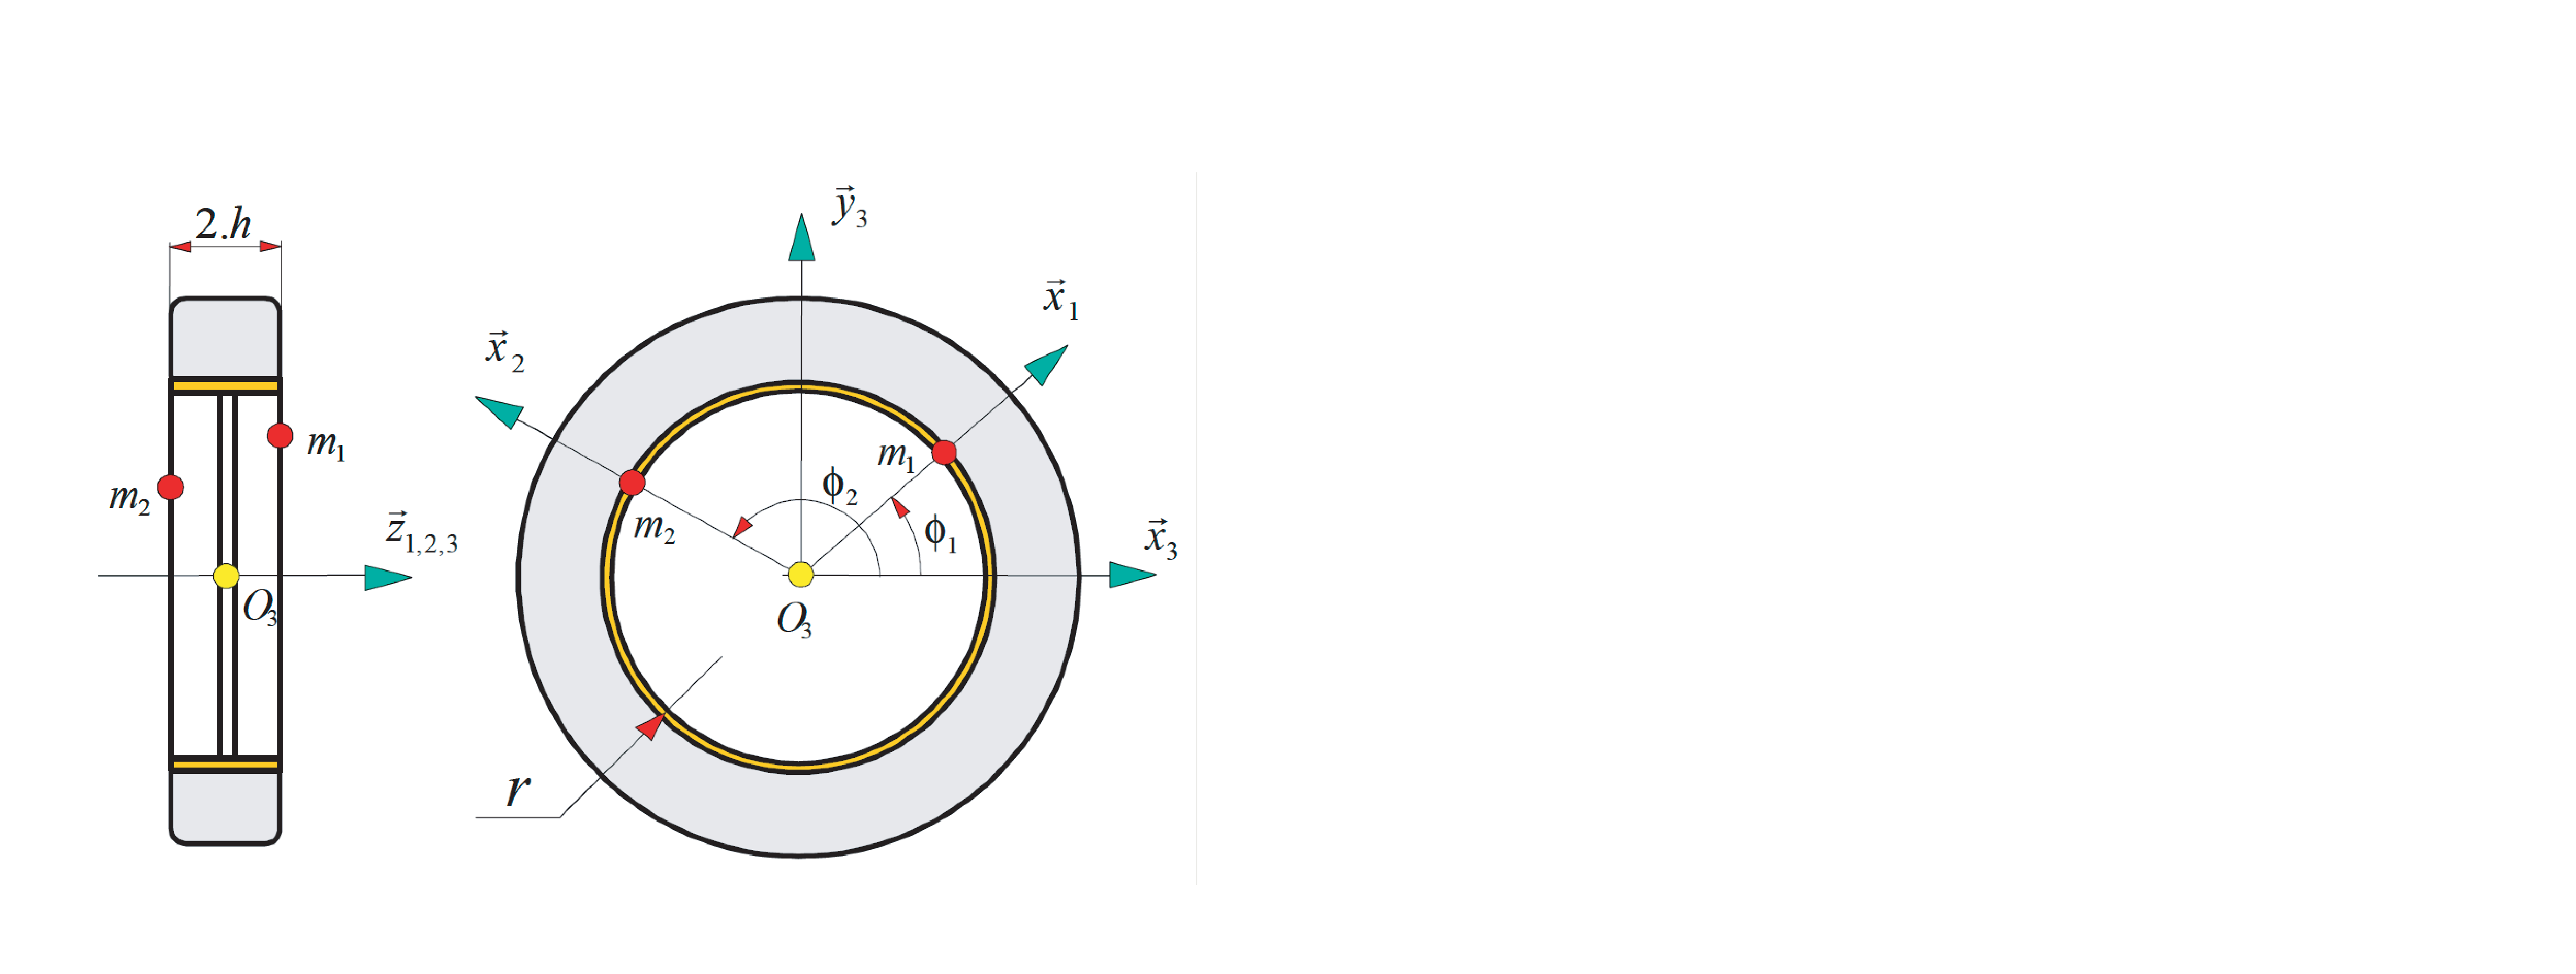
\includegraphics[width=0.9\textwidth]{images/figure-masse-roue.pdf}
\end{center}
\caption{Définition du problème avec la présence de masses d'équilibrage}
\end{figure}

On considère dorénavant l'ensemble cinématiquement lié $E=\left\{1+2+3\right\}$ : 
\begin{itemize}
\item Soit $G$ son centre d'inertie ;
\item $\overline{\overline{I}}{O_3}(E)$ sont opérateur d'inertie en $O_3$ :
$
\overline{\overline{I}}{O_3}(E)=
\left(\begin{array}{ccc}
A & -F & -E \\ 
-F & B & -D \\ 
-E & -D & C
\end{array} \right)_{R_3}
$.
\end{itemize}

\begin{exemple}[Détermination de l'équilibrage statique]
%\subparagraph{}
 \textit{Traduire la relation donnée par l'équilibrage statique.}
\begin{itemize}
\item La condition d'équilibrage statique implique : $\vect{O_3G} \vect{x_3}=0$ et $\vect{O_3G} \vect{y_3}=0$.
\item La formule du barycentre donne : 
%\begin{texteCache}
$
\vect{O_3G}=\frac{m_1 \vect{O_3G_1}+m_1 \vect{O_3G_2}+m_3 \vect{O_3G_3}}{m_1+m_2+m_3}.
$
%\end{texteCache}
\item On peut exprimer $\vect{O_3G_1}$ et $\vect{O_3G_2}$ dans la base $b_3=\base{{x_3}}{{y}_3}{{z}_{0,3}}$ :
%\begin{texteCache}
$$
\vect{O_3G_1}=r \cos\Phi_1 \vect{x_3}+r \sin\Phi_1 \vect{x_3}+h \vect{z_{0,3}}
\quad\quad\quad
\vect{O_3G_2}=r \cos\Phi_2 \vect{x_3}+r \sin\Phi_2 \vect{x_3}-h \vect{z_{0,3}}
$$

%\end{texteCache}
\item $\vect{O_3G} \vect{x_3}=0$ donne : 
%\begin{texteCache}
$
r \left(m_1 \cos\Phi_1+m_1 \cos\Phi_1 \right)=0$.
%\end{texteCache}
\item $\vect{O_3G} \vect{y_3}=0$ donne : 
%\begin{texteCache}
$
m_3 b+r \left(m_1 \sin\Phi_1+m_1 \sin\Phi_1 \right)=0
$.
%\end{texteCache}
\end{itemize}

%\subparagraph{}

\textit{Traduire la relation donnée par l'équilibrage dynamique.}

\begin{itemize}
\item L'opérateur d'inertie de $E$ en $O_3$ doit avoir la direction $\couple{O_3}{{z_{0,3}}}$  comme principale d'inertie d'où $D=E=0$.
\item On obtient alors une relation avec l'expression de $D$ : 
%\begin{texteCache}
$
D=D_3+m_1 y_1 z_1+ m_2 y_2 z_2=D_3+m_1 r \sin\Phi_1 h-m_2 r \sin\Phi_2 h
$.
%\end{texteCache}
\item On obtient alors une relation avec l'expression de $E$ :
%\begin{texteCache}
$E=E_3+m_1 x_1 z_1+m_2 x_2 z_2=E_3+m_1 r \cos\Phi_1 h-m_2 r \cos\Phi_2 h
$.
%\end{texteCache}
\end{itemize}

\end{exemple}

\subsection{Équations de détermination de l'équilibrage}

\begin{definition}[Équations de détermination de l'équilibrage]

En notant,
\begin{itemize}
\item $x_i$, $y_i$ et $z_i$ ($i$ allant de $1$ à $2$) les coordonnées des deux masselottes dans le repère $\quadruplet{O}{\vect{x_s}}{\vect{y_s}}{\vect{z_s}}$ lié à un solide $S$,
\item $r_s$ la distance entre le centre d'inertie de $S$ par rapport à $\couple{O}{{z}_s}$, 
\item $D_s$, $E_s$ et $E_s$ les produits d'inertie du solide S dans la base $b_s=\base{{x}_s}{{y}_s}{{z}_s}$
\end{itemize}
L'écriture des condition d'équilibrage d'un solide en rotation autour d'un axe $\couple{O}{{z}_s}$ donne : 

\begin{tabular}{|p{6.5cm}|p{6.5cm}|}
\hline 
\textbf{Centre d'inertie $G$ sur l'axe de rotation} & \textbf{Axe de rotation $\couple{O}{{z}}$ axe principal d'inertie du solide $S$} \\ 
\hline 
$m_1 x_1+m_2 x_2=0$
&
$D=D_s+m_1 y_1 z_1+ m_2 y_2 z_2$
\\ 
$m_3 r_s+m_1 y_1+m_2 y_2=0$
&
$E=E_s+m_1 x_1 z_1+m_2 x_2 z_2$\\
\hline 
\end{tabular} 

\end{definition}

\subsection{Mise en\ oe{}uvre : machine d'équilibrage industriel}

\begin{prop}[Mise en  \oe{}uvre de l'équilibrage dynamique]~\\

\begin{minipage}[c]{.8\linewidth}
D'après l'étude précédente, on obtient 4 équations avec 8 inconnues ($m_1$, $m_2$, $x_1$, $y_1$, $z_1$, $x_2$, $y_2$ et $z_2$).
Il faut donc imposer 4 variables. Généralement pour des raisons pratiques comme dans l'exemple précédent, on impose $z_1$ et $z_2$ puis on impose une relation entre $x_1$ et $y_1$ puis entre $x_2$ et $y_2$ cela revient à fixer une distance entre les masses additionnelles et l'axe de rotation.
Dans la pratique on utilise une équilibreuse qui mesure les efforts au niveau des paliers et qui en déduit les variables citées précédemment pour obtenir les conditions d'équilibrage.

\end{minipage}\hfill
\begin{minipage}[c]{.15\linewidth}
\begin{center}
\includegraphics[width=.9\linewidth]{images/machine_equilibrage.jpeg}
\end{center}
\end{minipage}
\end{prop}




\end{document}




